\documentclass[11pt,border=5pt]{standalone}
\usepackage{fontspec}
\setmainfont{cmunrm.otf}[BoldFont=cmunbx.otf,ItalicFont=cmunti.otf,BoldItalicFont=cmunbi.otf]
\usepackage{amsmath}
\usepackage{unicode-math}
\setmathfont{NewCMMath-Regular.otf}
\usepackage{tikz}
\usetikzlibrary{arrows.meta,patterns,angles,quotes}
\begin{document}
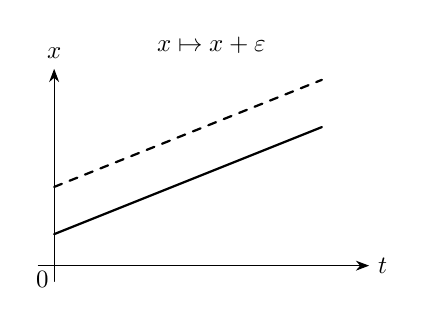
\begin{tikzpicture}[>=Stealth,font=\small,line cap=round,line join=round]
\draw[->,thin] (-0.2,0) -- (4,0) node[right] {$t$};
\draw[->,thin] (0,-0.2) -- (0,2.5) node[above] {$x$};
\node at (-0.14,-0.18) {$0$};
\draw[thick] plot coordinates {(0.00000,0.40000) (0.02833,0.41133) (0.05667,0.42267) (0.08500,0.43400) (0.11333,0.44533) (0.14167,0.45667) (0.17000,0.46800) (0.19833,0.47933) (0.22667,0.49067) (0.25500,0.50200) (0.28333,0.51333) (0.31167,0.52467) (0.34000,0.53600) (0.36833,0.54733) (0.39667,0.55867) (0.42500,0.57000) (0.45333,0.58133) (0.48167,0.59267) (0.51000,0.60400) (0.53833,0.61533) (0.56667,0.62667) (0.59500,0.63800) (0.62333,0.64933) (0.65167,0.66067) (0.68000,0.67200) (0.70833,0.68333) (0.73667,0.69467) (0.76500,0.70600) (0.79333,0.71733) (0.82167,0.72867) (0.85000,0.74000) (0.87833,0.75133) (0.90667,0.76267) (0.93500,0.77400) (0.96333,0.78533) (0.99167,0.79667) (1.02000,0.80800) (1.04833,0.81933) (1.07667,0.83067) (1.10500,0.84200) (1.13333,0.85333) (1.16167,0.86467) (1.19000,0.87600) (1.21833,0.88733) (1.24667,0.89867) (1.27500,0.91000) (1.30333,0.92133) (1.33167,0.93267) (1.36000,0.94400) (1.38833,0.95533) (1.41667,0.96667) (1.44500,0.97800) (1.47333,0.98933) (1.50167,1.00067) (1.53000,1.01200) (1.55833,1.02333) (1.58667,1.03467) (1.61500,1.04600) (1.64333,1.05733) (1.67167,1.06867) (1.70000,1.08000) (1.72833,1.09133) (1.75667,1.10267) (1.78500,1.11400) (1.81333,1.12533) (1.84167,1.13667) (1.87000,1.14800) (1.89833,1.15933) (1.92667,1.17067) (1.95500,1.18200) (1.98333,1.19333) (2.01167,1.20467) (2.04000,1.21600) (2.06833,1.22733) (2.09667,1.23867) (2.12500,1.25000) (2.15333,1.26133) (2.18167,1.27267) (2.21000,1.28400) (2.23833,1.29533) (2.26667,1.30667) (2.29500,1.31800) (2.32333,1.32933) (2.35167,1.34067) (2.38000,1.35200) (2.40833,1.36333) (2.43667,1.37467) (2.46500,1.38600) (2.49333,1.39733) (2.52167,1.40867) (2.55000,1.42000) (2.57833,1.43133) (2.60667,1.44267) (2.63500,1.45400) (2.66333,1.46533) (2.69167,1.47667) (2.72000,1.48800) (2.74833,1.49933) (2.77667,1.51067) (2.80500,1.52200) (2.83333,1.53333) (2.86167,1.54467) (2.89000,1.55600) (2.91833,1.56733) (2.94667,1.57867) (2.97500,1.59000) (3.00333,1.60133) (3.03167,1.61267) (3.06000,1.62400) (3.08833,1.63533) (3.11667,1.64667) (3.14500,1.65800) (3.17333,1.66933) (3.20167,1.68067) (3.23000,1.69200) (3.25833,1.70333) (3.28667,1.71467) (3.31500,1.72600) (3.34333,1.73733) (3.37167,1.74867) (3.40000,1.76000)};
\draw[thick,dashed] plot coordinates {(0.00000,1.00000) (0.02833,1.01133) (0.05667,1.02267) (0.08500,1.03400) (0.11333,1.04533) (0.14167,1.05667) (0.17000,1.06800) (0.19833,1.07933) (0.22667,1.09067) (0.25500,1.10200) (0.28333,1.11333) (0.31167,1.12467) (0.34000,1.13600) (0.36833,1.14733) (0.39667,1.15867) (0.42500,1.17000) (0.45333,1.18133) (0.48167,1.19267) (0.51000,1.20400) (0.53833,1.21533) (0.56667,1.22667) (0.59500,1.23800) (0.62333,1.24933) (0.65167,1.26067) (0.68000,1.27200) (0.70833,1.28333) (0.73667,1.29467) (0.76500,1.30600) (0.79333,1.31733) (0.82167,1.32867) (0.85000,1.34000) (0.87833,1.35133) (0.90667,1.36267) (0.93500,1.37400) (0.96333,1.38533) (0.99167,1.39667) (1.02000,1.40800) (1.04833,1.41933) (1.07667,1.43067) (1.10500,1.44200) (1.13333,1.45333) (1.16167,1.46467) (1.19000,1.47600) (1.21833,1.48733) (1.24667,1.49867) (1.27500,1.51000) (1.30333,1.52133) (1.33167,1.53267) (1.36000,1.54400) (1.38833,1.55533) (1.41667,1.56667) (1.44500,1.57800) (1.47333,1.58933) (1.50167,1.60067) (1.53000,1.61200) (1.55833,1.62333) (1.58667,1.63467) (1.61500,1.64600) (1.64333,1.65733) (1.67167,1.66867) (1.70000,1.68000) (1.72833,1.69133) (1.75667,1.70267) (1.78500,1.71400) (1.81333,1.72533) (1.84167,1.73667) (1.87000,1.74800) (1.89833,1.75933) (1.92667,1.77067) (1.95500,1.78200) (1.98333,1.79333) (2.01167,1.80467) (2.04000,1.81600) (2.06833,1.82733) (2.09667,1.83867) (2.12500,1.85000) (2.15333,1.86133) (2.18167,1.87267) (2.21000,1.88400) (2.23833,1.89533) (2.26667,1.90667) (2.29500,1.91800) (2.32333,1.92933) (2.35167,1.94067) (2.38000,1.95200) (2.40833,1.96333) (2.43667,1.97467) (2.46500,1.98600) (2.49333,1.99733) (2.52167,2.00867) (2.55000,2.02000) (2.57833,2.03133) (2.60667,2.04267) (2.63500,2.05400) (2.66333,2.06533) (2.69167,2.07667) (2.72000,2.08800) (2.74833,2.09933) (2.77667,2.11067) (2.80500,2.12200) (2.83333,2.13333) (2.86167,2.14467) (2.89000,2.15600) (2.91833,2.16733) (2.94667,2.17867) (2.97500,2.19000) (3.00333,2.20133) (3.03167,2.21267) (3.06000,2.22400) (3.08833,2.23533) (3.11667,2.24667) (3.14500,2.25800) (3.17333,2.26933) (3.20167,2.28067) (3.23000,2.29200) (3.25833,2.30333) (3.28667,2.31467) (3.31500,2.32600) (3.34333,2.33733) (3.37167,2.34867) (3.40000,2.36000)};
\node at (2,2.8) {$x\mapsto x+\varepsilon$};

\end{tikzpicture}
\end{document}
